\documentclass{article}

\usepackage[czech]{babel}
\usepackage[a4paper]{geometry}
\usepackage{amsmath}
\usepackage{graphicx}
\PassOptionsToPackage{hyphens}{url}\usepackage{hyperref}

\begin{document}
\begin{titlepage}
		\begin{center}
			\Huge\textsc{Vysoké učení technické v~Brně} \\
			\huge\textsc{Fakulta informačních technologií} \\
			\vspace{\stretch{0.4}}
			\LARGE IMP\,--\,projekt \\
			\Huge ESP32: Měření srdečního tepu [digitální senzor] 
			\vspace{\stretch{0.6}}
		\end{center}


		{\Large
			\today\hfill
			Rostislav Král
		}
	\end{titlepage}

\section{O projektu}
V tomto projektu měl být implementován měřič srdečního tepu za pomocí MCU ESP32, digitálního senzoru MAX30102 a OLED displeje. Byly použity aplikační rámce ESP-IDF a komponenta pro SSD1306. Projekt implementuje "pouze"  měření tepu.
\section{Popis HW}
Řešení využívá rozhraní SPI pro komunikaci s OLED displejem a zapojení je následující:

\begin{itemize}
    \item GND $---->$ GND
    \item VCC $---->$ 3.3V
    \item SCK $---->$ GPIO 18
    \item MOSI $---->$ GPIO 23
    \item RES $---->$ GPIO 17
    \item DC $---->$ GPIO 16
    \item CS $---->$ GPIO 5
\end{itemize}

Senzor MAX30102 je zapojen takto(I2C komunikace):

\begin{itemize}
    \item GND $---->$ GND
    \item VCC $---->$ 3.3V
    \item SCL $---->$ GPIO 32
    \item SDA $---->$ GPIO 33

\end{itemize}

\section{Implementace}
V projektu bylo nutné si nastavit I2C mastera, dále potom správně nastavit registry senzoru MAX30102 z datasheetu \url{https://www.analog.com/media/en/technical-documentation/data-sheets/MAX30102.pdf}, a pro něj implementovat funkce pro čtení hodnot z LED. Vzorkovací frekvence je nastavena na 25Hz, počet vzorků pro jedno měření pak na 128. Dále bylo nutné naimplementovat vlastní filtry signálu, používá se dolní propust pro vyhlazení, poté jsou ještě hodnoty vyfiltrované/znormalizované průměrem signálu. Následně funkce pro autokorelaci a detekci vrcholů v korelovaném signálu, jejich porovnání: (za referenční jsem považoval implementaci knihovny Scipy, viz. grafy \ref{fig:signals}, hodnoty jsou z \ref{fig:debug}). Většinou se pohybujeme v celých číslech. Displej je ovládán pomocí rozhraní z \url{https://github.com/nopnop2002/esp-idf-ssd1306}. 

$$
    R(k) = \sum_{n=0}^{N-k-1}x[n]*x[n+k]
$$
Kde R(k) je hodnota autokorelačního koeficientu, N počet vzorků, k offset a x[n] vstupní signál.

Výpočet BPM je potom definován jako: $BPM = 60/T$, kde T je perioda v sekundách vyjadřena jako $ T = peak/f_s $

Video dostupné zde: \url{https://drive.google.com/file/d/1ye9kaQlFNYgUjggz3Z9idHxatKQFFrNM/view?usp=sharing}
\section{Závěr}
Projekt funguje celkem dobře, známé problémy jsou např. špatné umístění prstu na senzor, kdy je signál zkreslen anebo nepřenost výpočtu, jelikož projekt používá většinou pouze celá čísla a ne úplně komplexní algoritmy pro práci se signály(i tak jsou ale výsledky dostatečně přesné). 
\section{Autoevaluace}
\begin{itemize}
    \item E = 2 (ESP-IDF, vlastní zpracovaní signálu)
    \item F = 5 (Projekt je funkční, ověřeno s komerčním meřičem viz. video)
    \item Q = - (Nedokážu zhodnotit)
    \item P = 2 
    \item D = 3 (\LaTeX, myslím si, že je vše dostatečně zdokumentováno)
\end{itemize}



\begin{figure}
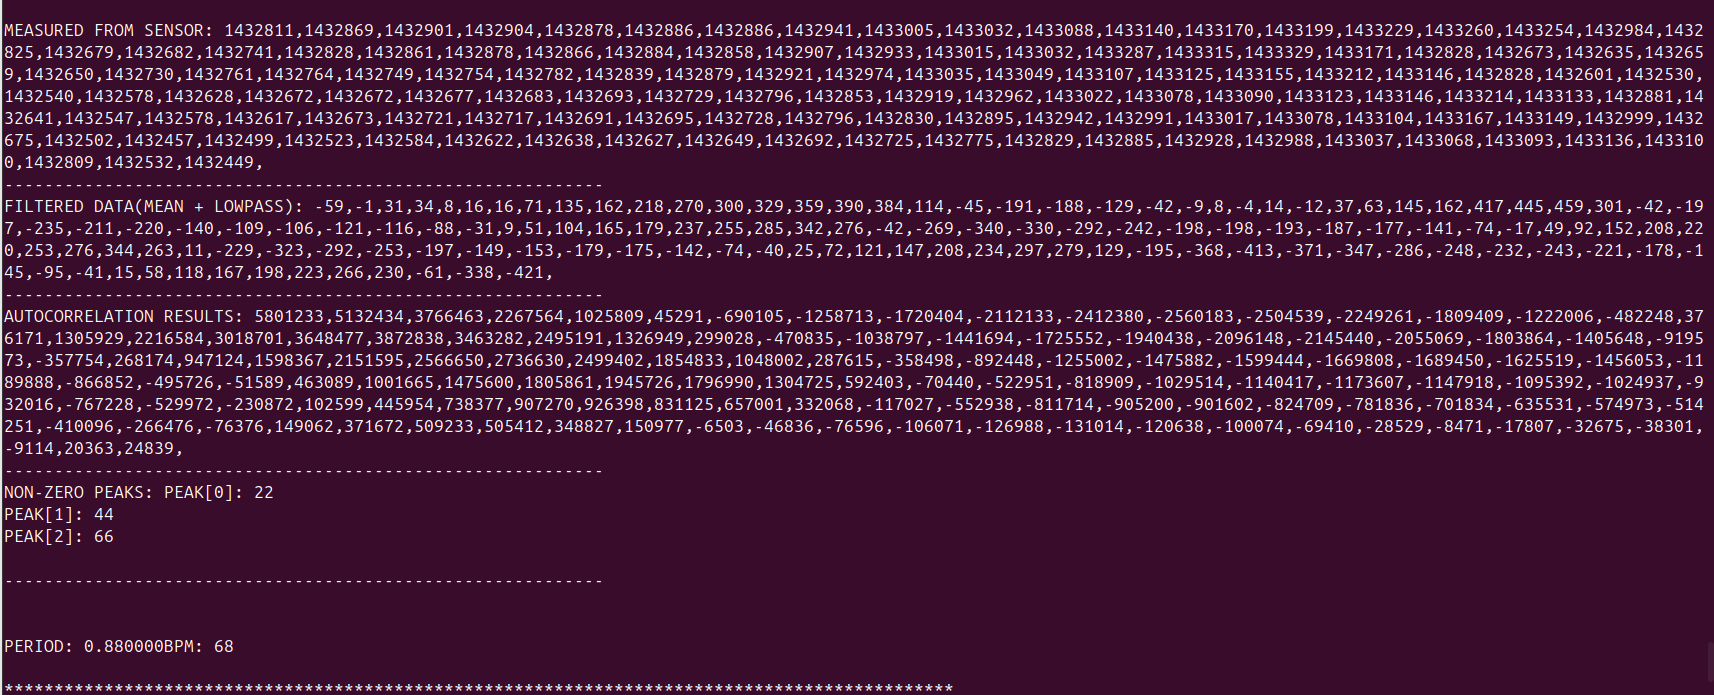
\includegraphics[width=\linewidth]{debug.png}
\caption{\label{fig:debug}Debug z ESP a senzoru, použito pro grafy v \ref{fig:signals}}
\end{figure}


\begin{figure}
\label{signals}
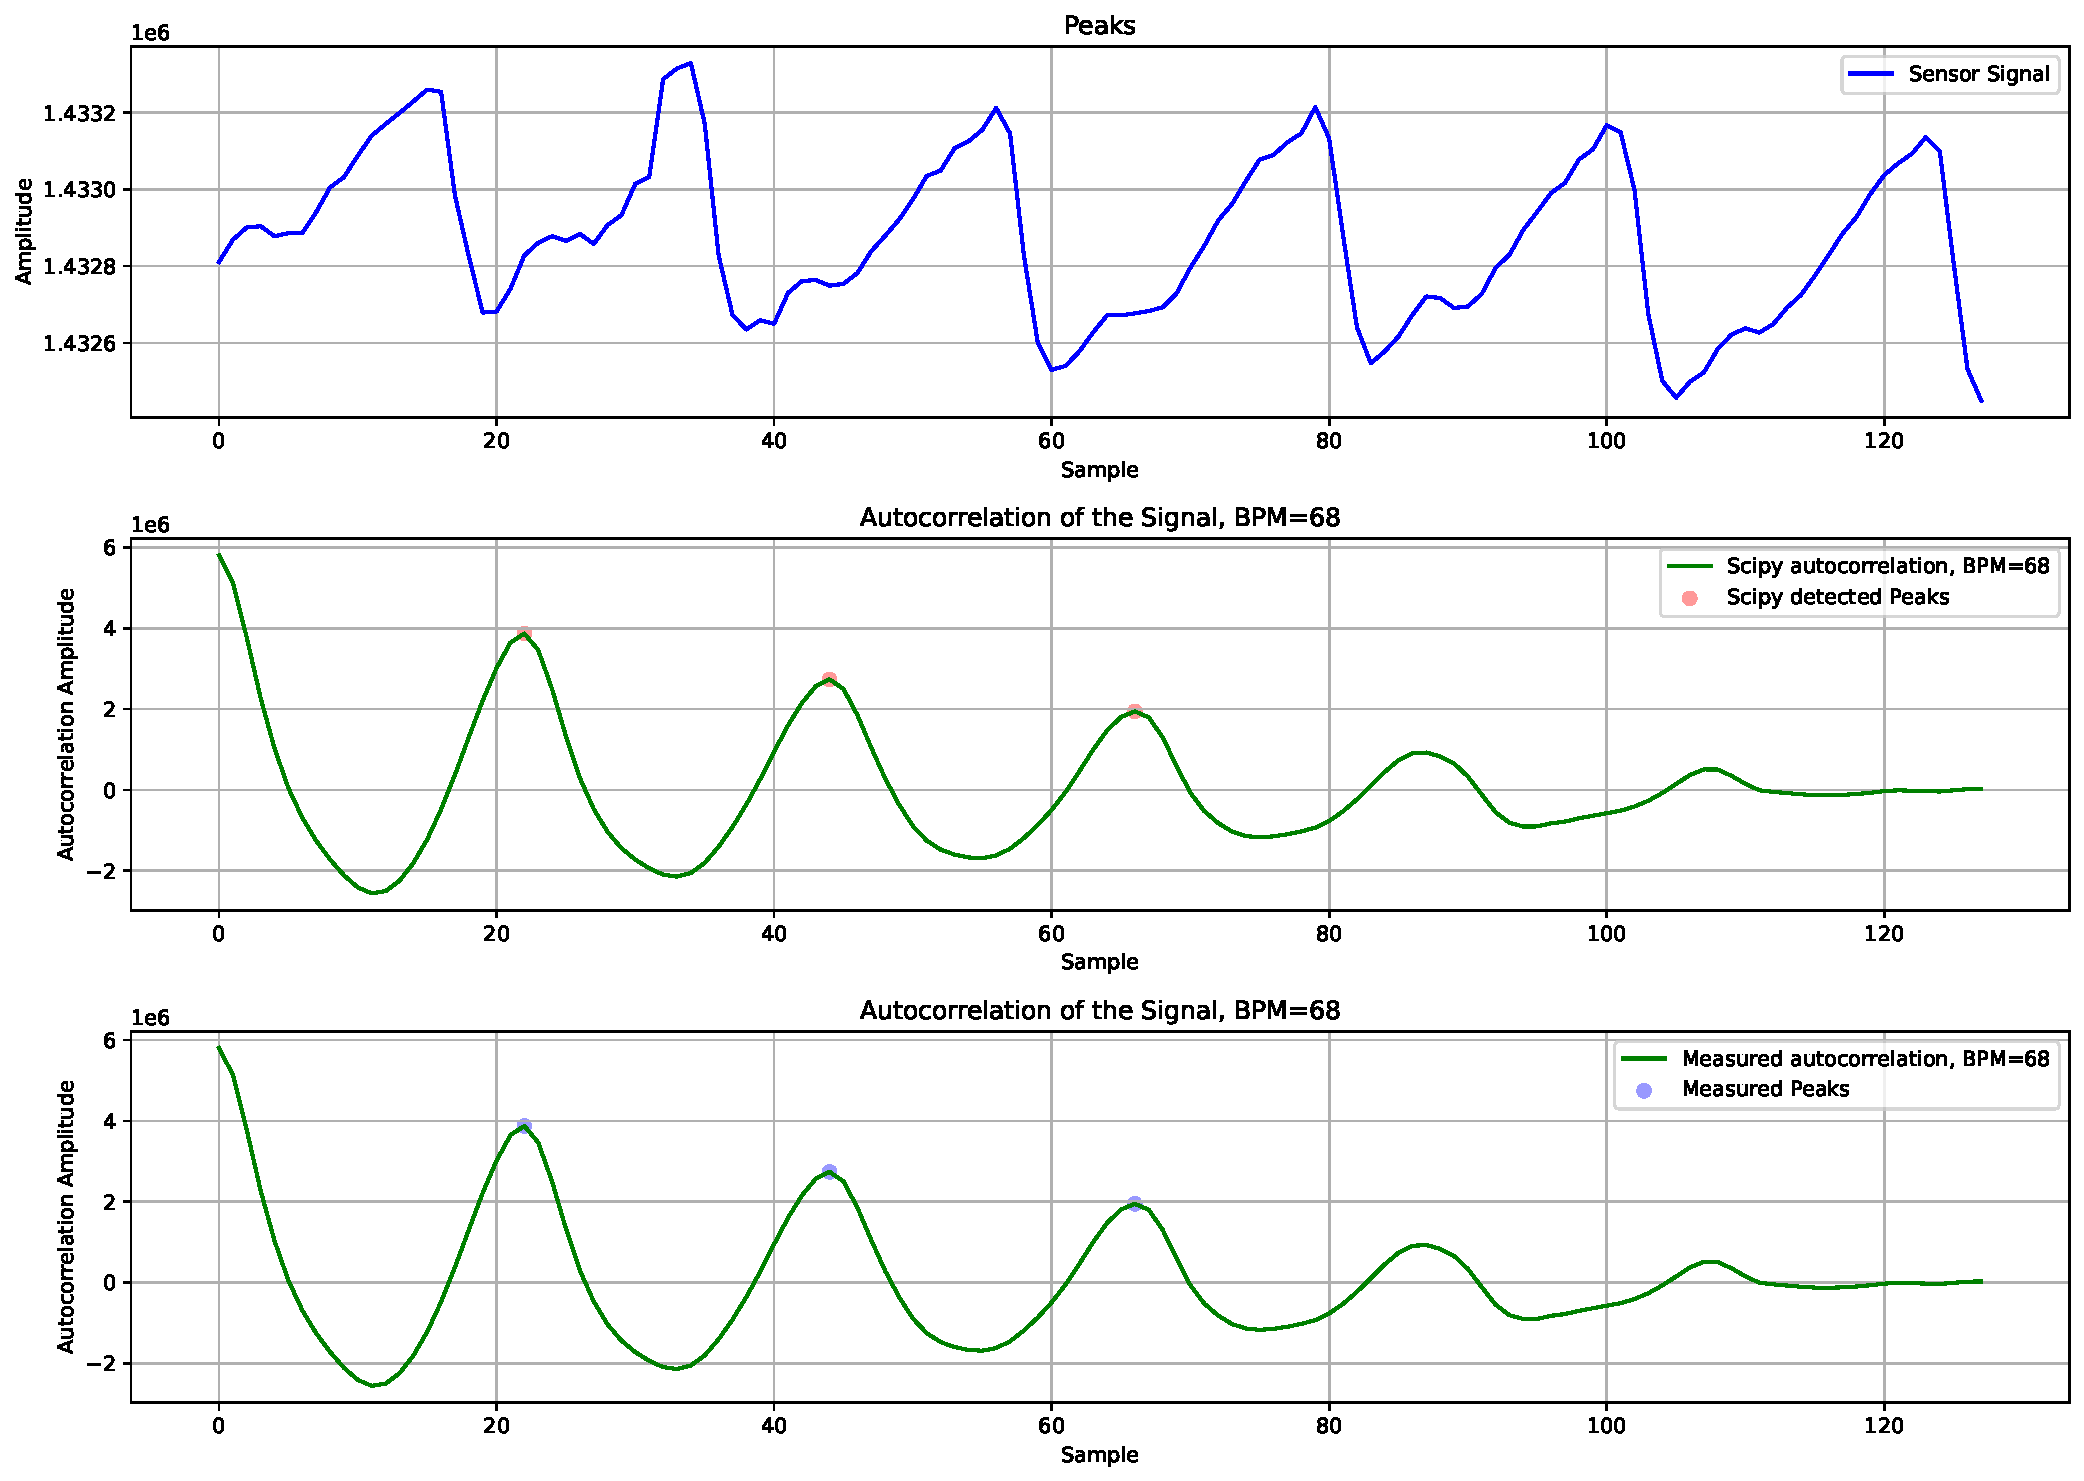
\includegraphics[width=\linewidth]{signals.pdf}
\caption{\label{fig:signals}Scipy vs naměřené hodnoty}
\end{figure}



\end{document}